\subsubsection{Activation of a perceptron} \label{subs:acti}
In order to decide if a perceptron is activated or not (if its threshold is reached), an activation function needs to be defined. However, to use this function in a \acrshort{dl} model and be able to apply the back-propagation algorithm (will be further detailed in Section \ref{subsec:train}), this function needs to be differentiable \cite{lecun_backpropagation_1989}. Indeed, during the optimization of the network, the gradient of the activation function is computed. Therefore, Equation \ref{eq:step} cannot be used as the activation function because of its zero gradient and the learning does not converge.  Various activation functions have been proposed with different properties, as illustrated in Figure \ref{fig:acti}. According to \textcite{khan_survey_2020}, the choice of an appropriate activation function can accelerate the learning phase and some activations decrease the computational complexity \cite{krizhevsky_imagenet_2012}.
%
\begin{figure}[H]
    \centering
    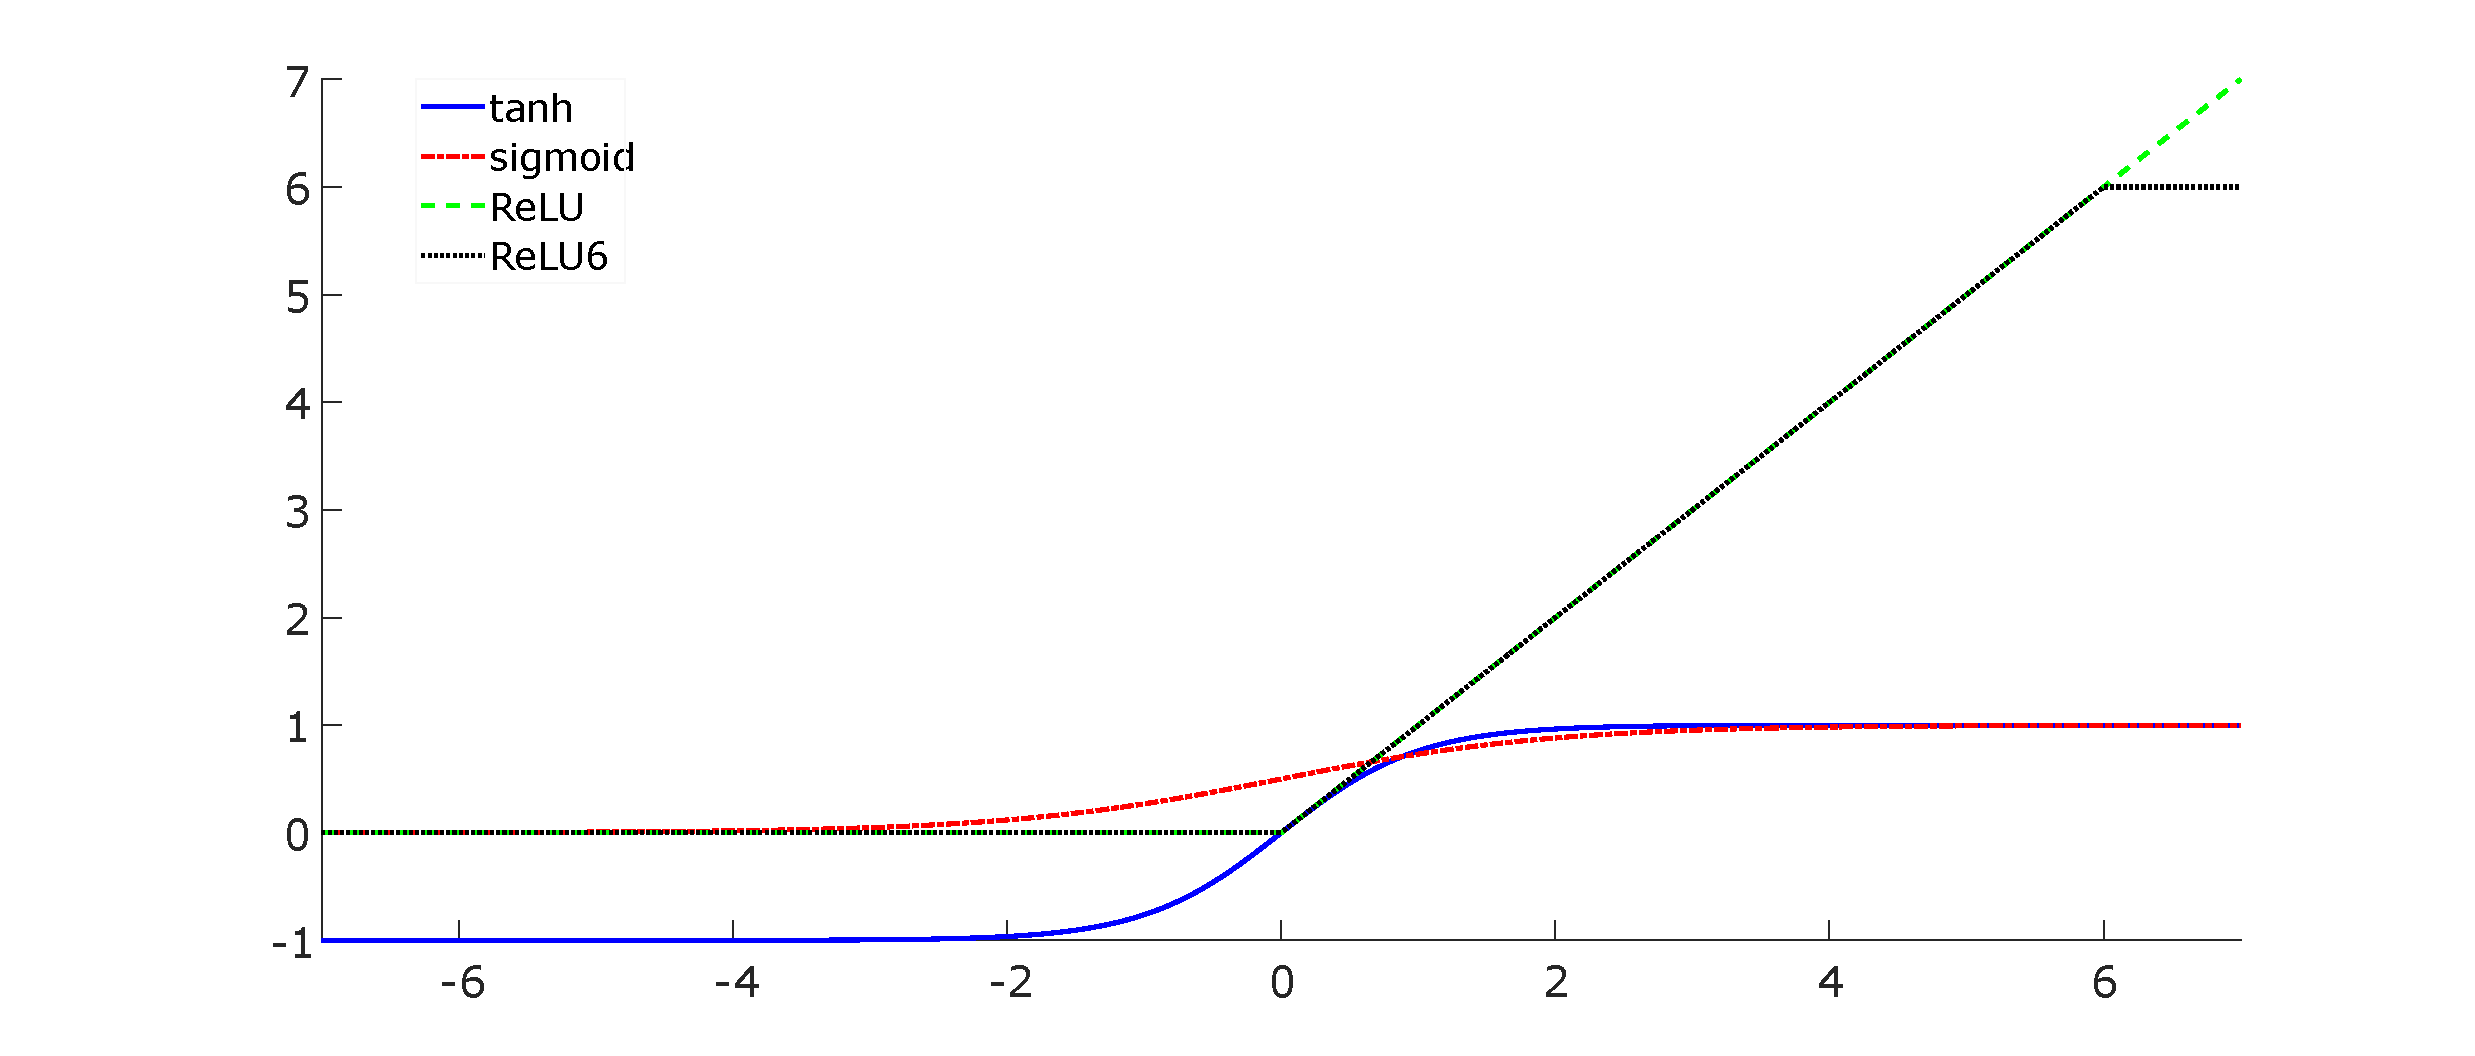
\includegraphics[width=0.85\textwidth]{actifun.pdf}
    \caption{Activation functions}
    \label{fig:acti}
\end{figure}
%
\subsubsection{Sigmoid and Hyperbolic Tangent (Tanh)}
$Sigmoid$ and $Tanh$ are smooth activation functions that limith the $\mathbb{R}$ domain into a narrower domain, $[0, 1]$ for $Sigmoid$, and $[-1, 1]$ for the $Tanh$, as shown in Figure \ref{fig:acti} \cite{matteucci_artificial_2019}. Therefore, they can be described using Equations \eqref{eq:sigmoid} and \eqref{eq:tanh} \cite{krizhevsky_imagenet_2012}.
%
\begin{equation}
    h(x) = \frac{1}{1 + e^{-x}}
    \label{eq:sigmoid}
\end{equation}
%
\begin{equation}
    h(x) = \frac{e^{x} - e^{-x}}{e^{x} + e^{-x}}
    \label{eq:tanh}
\end{equation}
%
However, they saturate at the asymptotes, which means that often their gradient is close to 0 \cite{glorot_understanding_2010}. As the back-propagation algorithm (see Section \ref{subsec:train}) requires gradient multiplication, gradient far away from the output vanishes (close to 0) and deep models do not learn. It is the \textbf{vanishing gradient problem} \cite{khan_survey_2020, goodfellow_deep_2016, matteucci_artificial_2019, maas_rectier_2013}.
%
\subsubsection{ReLU}
In order to overcome this vanishing gradient problem, the Rectified Linear Unit (ReLU) which is defined by Equation \eqref{eq:relu} has been developed by \textcite{krizhevsky_imagenet_2012}.
%
\begin{equation}
    h(x) = max(0, x)
    \label{eq:relu}
\end{equation}
%
This function increases the learning and computational speed compared to the $Tanh$ and $Sigmoid$ functions and improves the propagation gradient efficiency (to avoid vanishing or exploding gradient) \cite{maas_rectier_2013, abdelouahab_accelerating_2018}. However, in this function, some perceptrons can become inactive which means that their output is zero for all input. It is called the \textbf{dying neuron problem} which decreases the model capacity \cite{matteucci_artificial_2019}. A solution would be to discard these inactive neurons by transforming the ReLU into a leaky ReLU \cite{maas_rectier_2013} activation function for example.

We can also use the dying neuron property to learn sparse features earlier. It has been done by \textcite{krizhevsky_convolutional_2010} by setting an upper bound to the ReLU output. For example, in the work, the output is described by Equation \eqref{eq:relu6} and this activation function is called ReLU6 because the range is limited to $[0, 6]$. ReLU has also the advantage to be designed for fixed-point operations and quantization approaches (which will be more described in Section \ref{subsec:mdopti}), instead of floating-point operations. Indeed, floating-point operations, especially on \acrshort{fpga}, are less efficient in terms of hardware utilization and power consumption \cite{david_hardware_2007}. It means that if for example the output $ \in [0, 6]$, the number of bits for the integer part can be limited to 3 bits. The accuracy of the model can thus be increased by assigning the other available bits to the decimal part. For example, ReLU6 is used in model that aims mobile and embedded platforms like MobileNet \cite{howard_mobilenets_2017}. In this work, the ReLU6 activation function is used.
%
\begin{equation}
    h(x) = max(0, x, 6)
    \label{eq:relu6}
\end{equation}
